\chapter{Deployment}
\section{Google Play Store}
This section will dive into the development and administrative tasks required to officially deploy the app to the public. This task only commenced once Beta Testing was declared complete. Recall the way we managed app releases through Alpha and Beta testing, deployment to production was done in a very similar way. The Android Developer Console facilitiated this task through a "Push to Production" button on the latest beta release of the app.
Before the app was pushed to production, a series of forms and administrative tasks were required. 

Firstly, an app title and descriptions were needed (Figure \ref{fig:appdetailsform}). These would be displayed on the app's download page, with the goal of persuading the user to click on the app and download it. After testing stages, it was decided to add the "Free Skin Cancer Tracker" label to the name. This is purely an advertisement instrument to ensure the app appears in as many searches as possible.

Secondly, the app's nature required the creation of a privacy policy (Figure \ref{fig:privacypolicy}). This is usually optional, but apps that require storage or camera permissions have to include one. An app privacy policy generator \cite{nishantsrivastava} was used for this task. The file was hosted on a \emph{Github} website repository to ensure it was permanently available.

Thirdly, the app's pricing details had to be defined (Figure \ref{fig:apppricing}). As determined previously, the app would follow a free business model, with no in app purchases or ads either. All 144 available countries would be included in the deployment list.

In fourth place, a content rating questionnaire had to be filled in (Figure \ref{fig:contentrating}). App content ratings intend to help parents identify potentially objectionable content that exists within an app. In the case of our app, the PEGI 3 age tag was delivered, this means Google determined the app to be suitable for all age groups.

Lastly, the app's graphics had to be uploaded (Figure \ref{fig:appscreenshots}). An app's graphics include:
\begin{itemize}
    \item App screenshots
    \item Highest resolution icon
    \item Feature graphic (banner)
\end{itemize}
The icon and banner were designed with the Inkscape vector graphics editor, combining different layers of copyright-free cliparts.

Once all the described forms were complete, the app was submitted to the Google Play Store. Four hours later, the app was successfully approved and officially deployed (Figure \ref{fig:applisting}). If you recall the app listing screenshot from Beta testing (Figure \ref{fig:betarelease}), the app title had an "(Unreleased)" tag. This tag is no longer shown.

\begin{figure}
    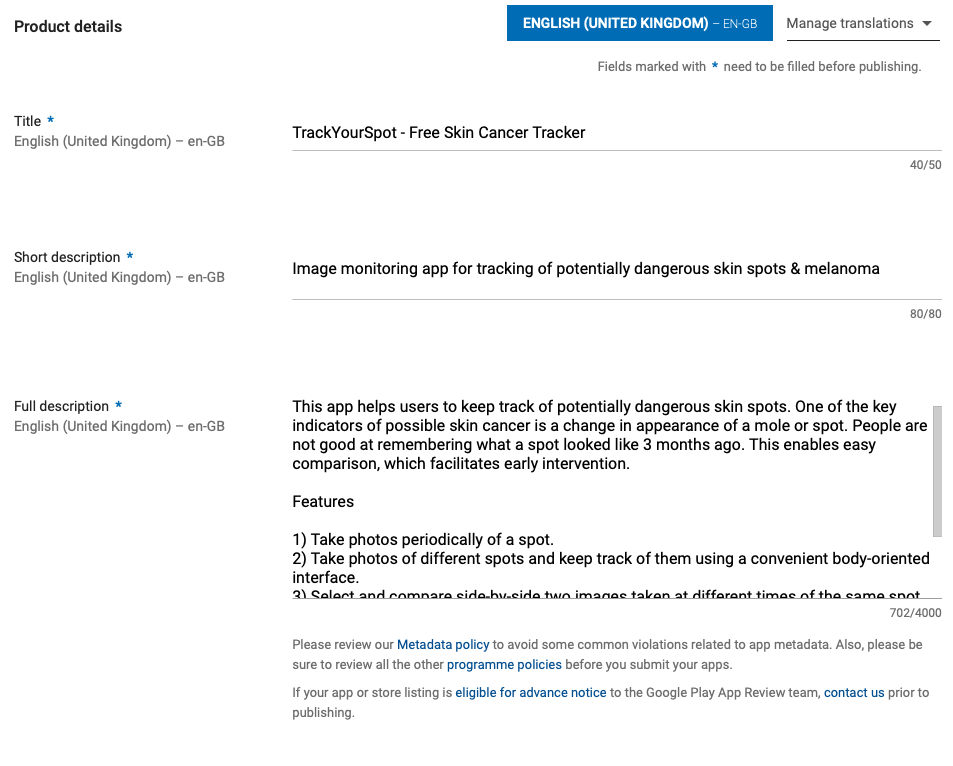
\includegraphics[width=1\textwidth, center]{figures/appnaming.png}
    \caption{Google Play Store App Details}
    \label{fig:appdetailsform}
\end{figure}

\begin{figure}
    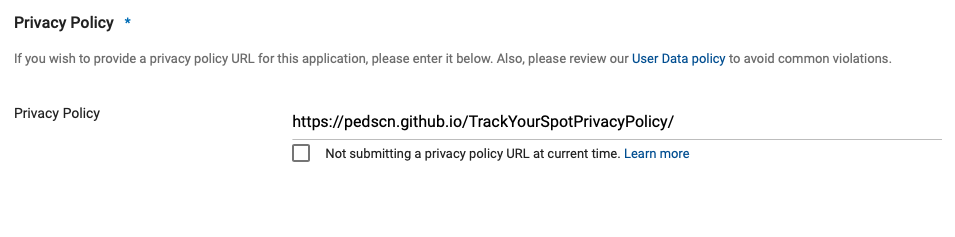
\includegraphics[width=1\textwidth, center]{figures/appprivacypolicy.png}
    \caption{Google Play Store Privacy Policy Form}
    \label{fig:privacypolicy}
\end{figure}

\begin{figure}
    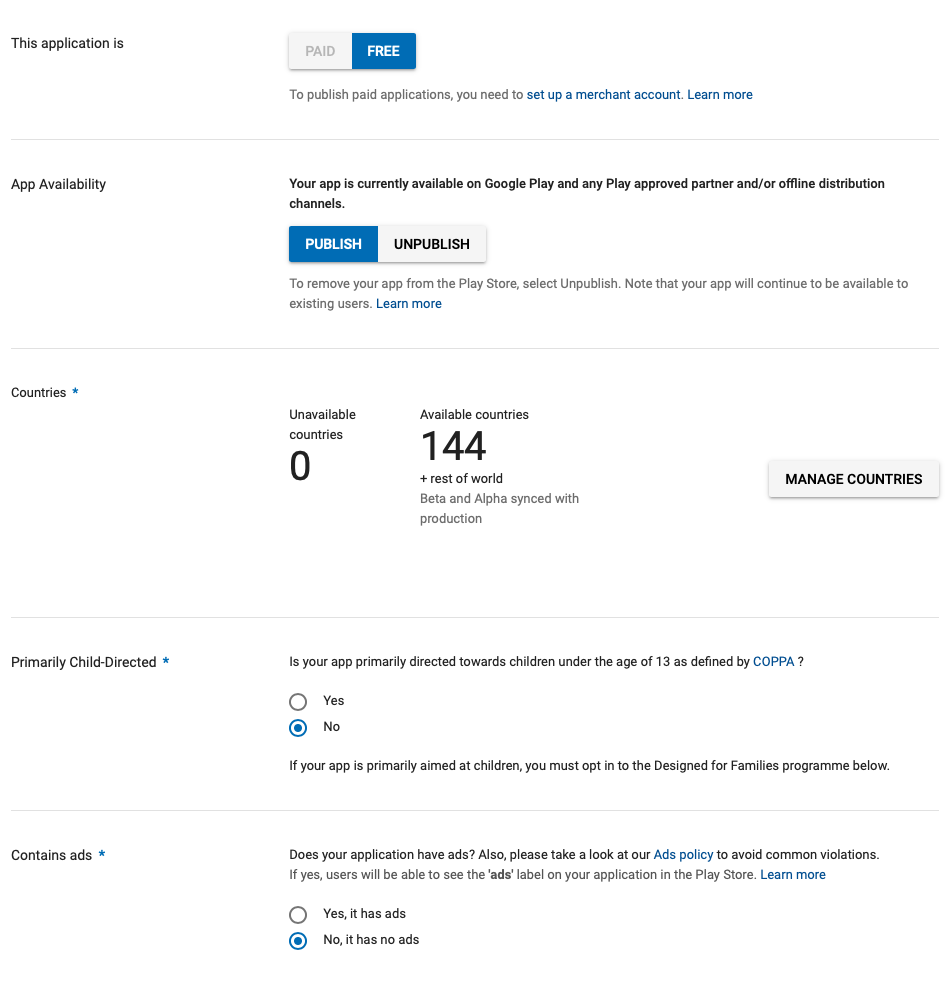
\includegraphics[width=1\textwidth, center]{figures/apppricing.png}
    \caption{\emph{TrackYourSpot} Deployment Settings}
    \label{fig:apppricing}
\end{figure}

\begin{figure}
    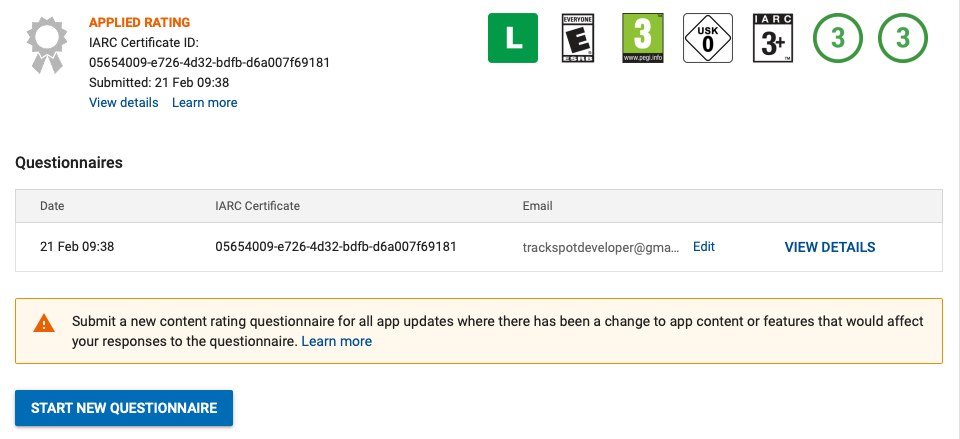
\includegraphics[width=1\textwidth, center]{figures/appcontentrating.png}
    \caption{Google Play Store Content Rating}
    \label{fig:contentrating}
\end{figure}

\begin{figure}
    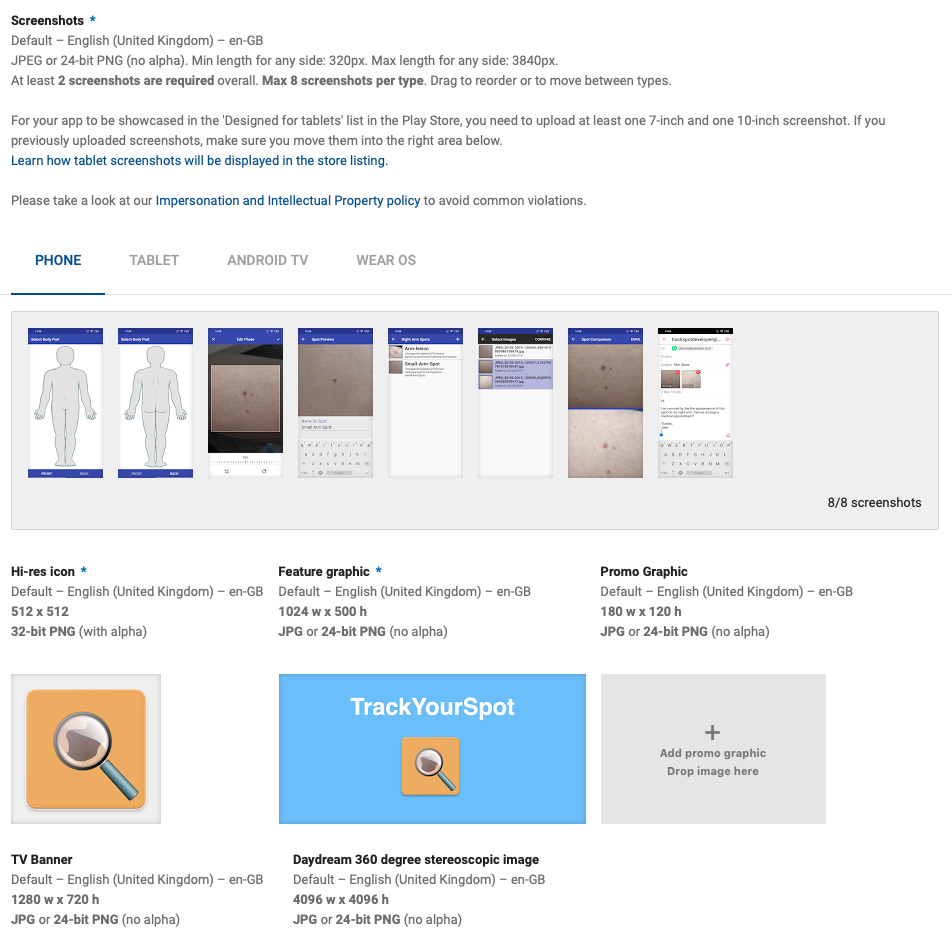
\includegraphics[width=1\textwidth, center]{figures/appscreenshots.png}
    \caption{Google Play Store Image Uploads}
    \label{fig:appscreenshots}
\end{figure}

\begin{figure}
    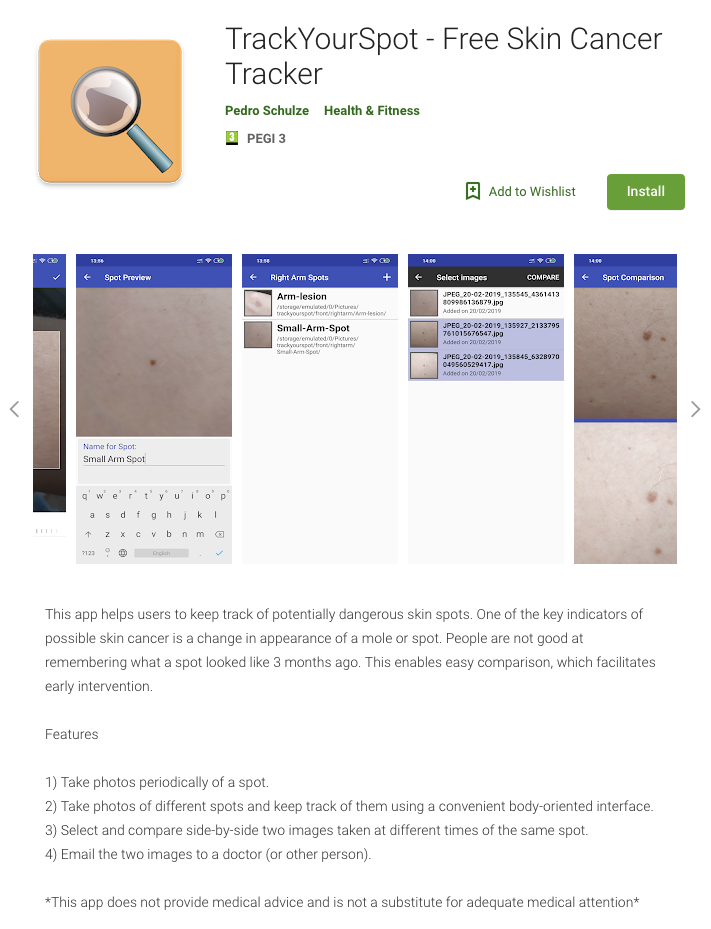
\includegraphics[width=1\textwidth, center]{figures/applisting.png}
    \caption{\emph{TrackYourSpot} app officially available to the public}
    \label{fig:applisting}
\end{figure}

\section{Website}
As part of the project, a website had to be developed to provide guidance on how to carry out all the core tasks of the app. To get started, a \emph{Bootstrap} business website template was downloaded from \emph{StartBootstrap} \cite{bootstrap}. Bootstrap is an HTML, CSS and Javascript framework to develop responsive websites \cite{twbs_2019}. This template was adapted to include links for all the tasks to be explained. Links for the Google Play Store and Android App Store versions of the app were also included. Figures \ref{fig:webdeployhome} - \ref{fig:webdeployadd} show a selection of screenshots of the finished website. The full website can be found at \code{www.trackyourspot.com}. 

This part of the project was also done by the iOS \emph{TrackYourSpot} developer, my contributions are described below: 
\begin{itemize}
    \item Page formatting and design of the home screen
    \item Finding suitable copyright free cliparts to be used as icons for the home screen (Figure \ref{fig:webdeployhome2}) 
    \item Modifying HTML code to describe steps to be completed for multiple tasks
    \item Attaching Android screenshots for each step
\end{itemize}


\begin{figure}
    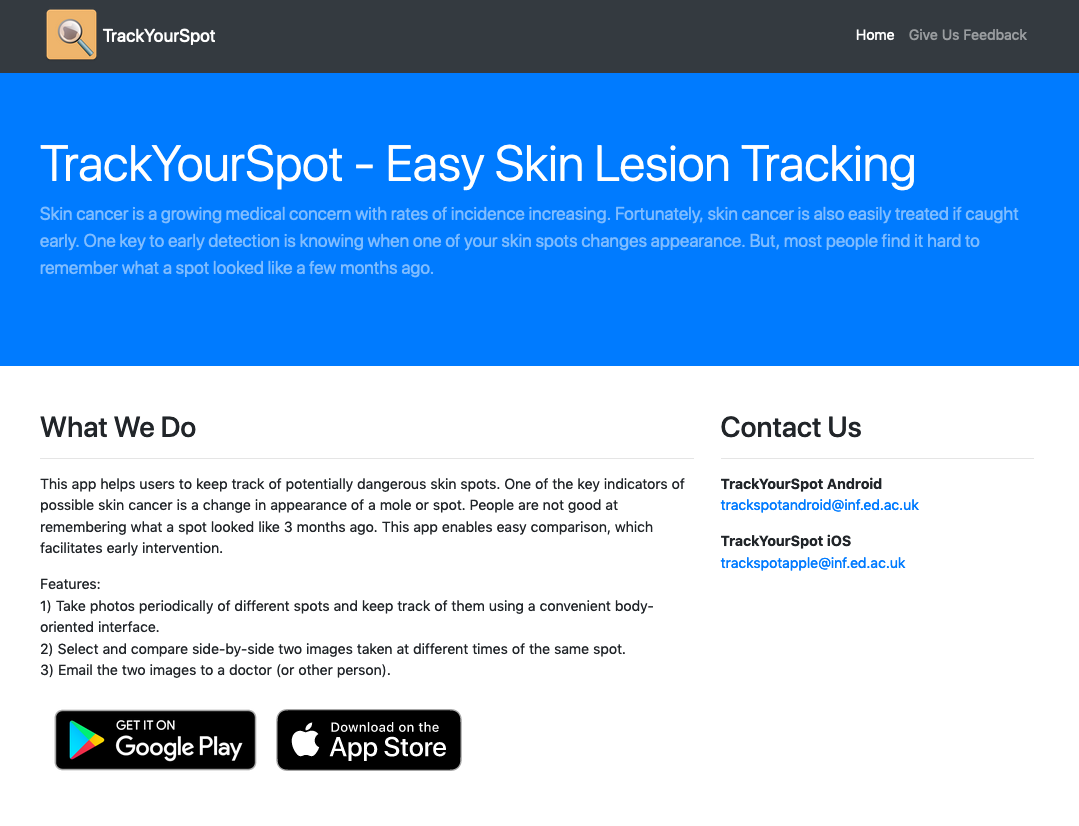
\includegraphics[width=1\textwidth, center]{figures/webdeployhome.png}
    \caption{\emph{TrackYourSpot} website homepage}
    \label{fig:webdeployhome}
\end{figure}

\begin{figure}
    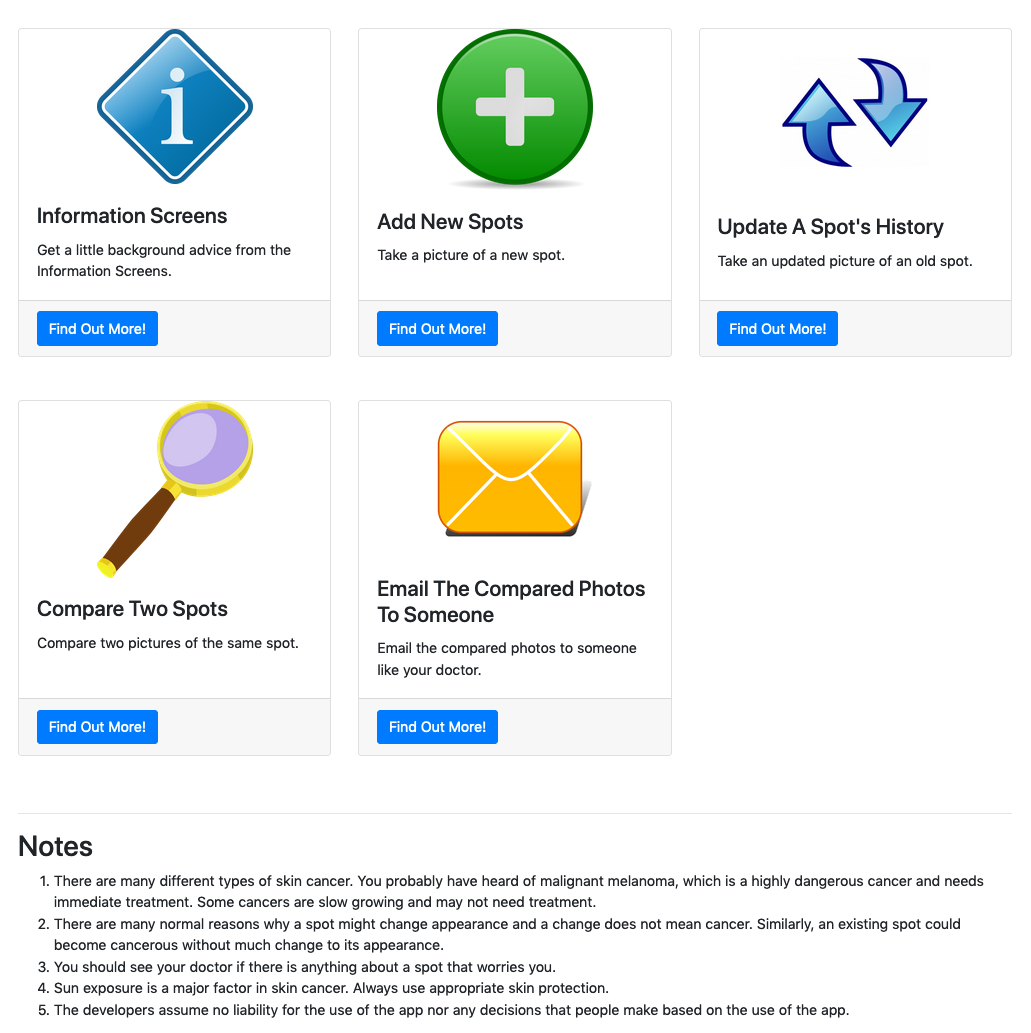
\includegraphics[width=1\textwidth, center]{figures/webdeployhome2.png}
    \caption{\emph{TrackYourSpot} website homepage (continued)}
    \label{fig:webdeployhome2}
\end{figure}

\begin{figure}
    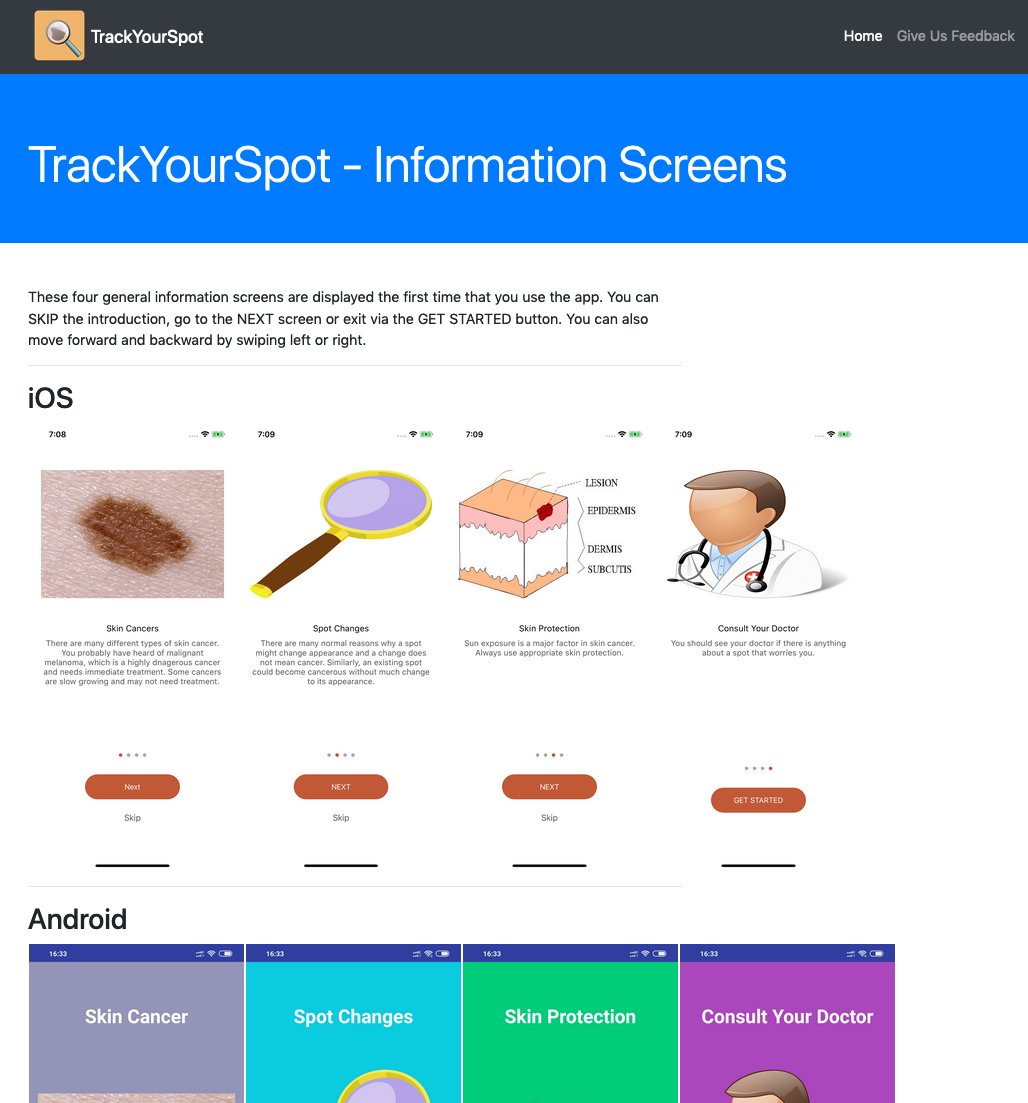
\includegraphics[width=1\textwidth, center]{figures/webdeployinfo.png}
    \caption{\emph{TrackYourSpot} website information screens guidance}
    \label{fig:webdeployinfo}
\end{figure}

\begin{figure}
    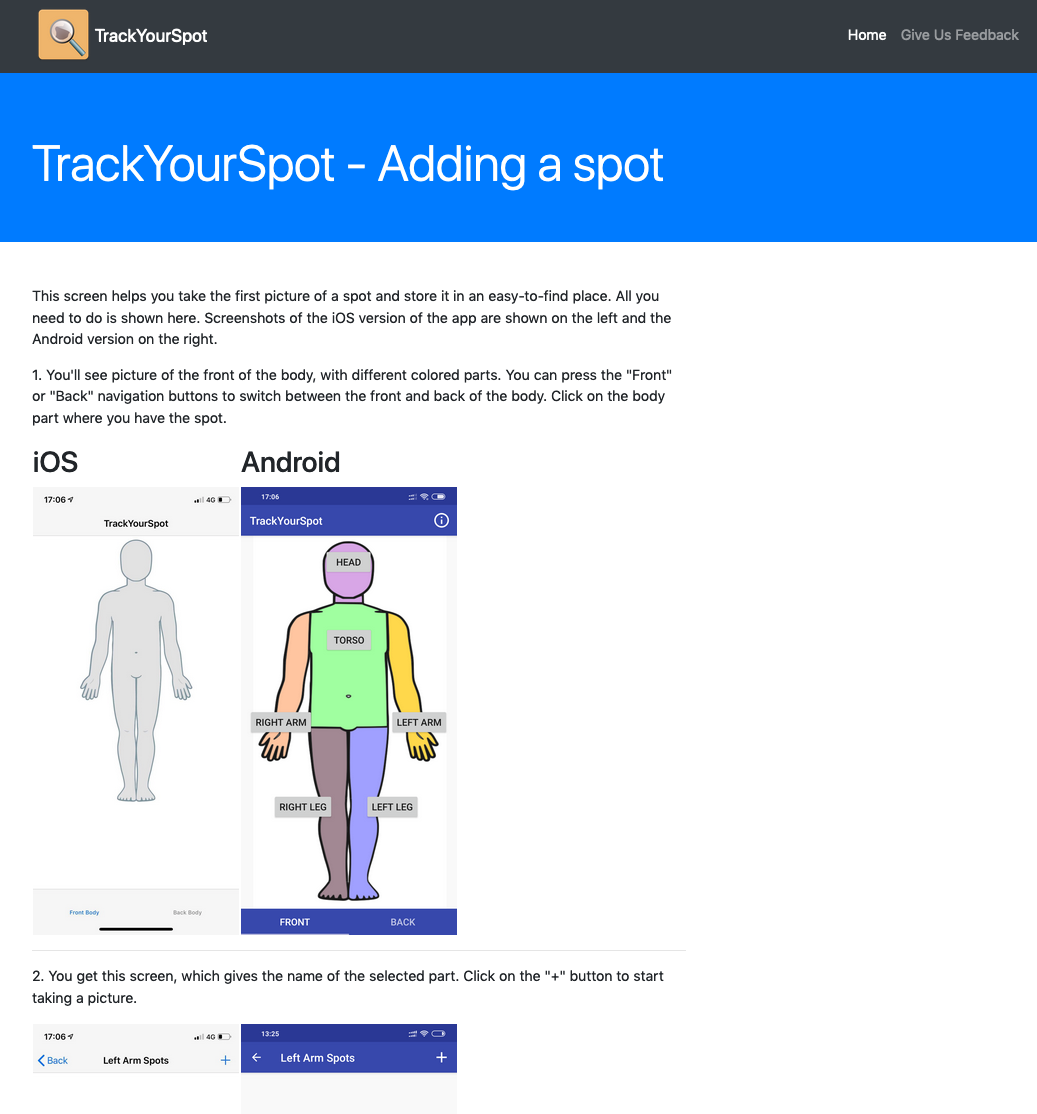
\includegraphics[width=1\textwidth, center]{figures/webdeployadd.png}
    \caption{\emph{TrackYourSpot} website adding a spot guidance}
    \label{fig:webdeployadd}
\end{figure}


